\documentclass[tikz,border=3pt]{standalone}
\usepackage{amsmath}
\usepackage{tikz}
\usetikzlibrary{arrows.meta,patterns,calc}

\begin{document}
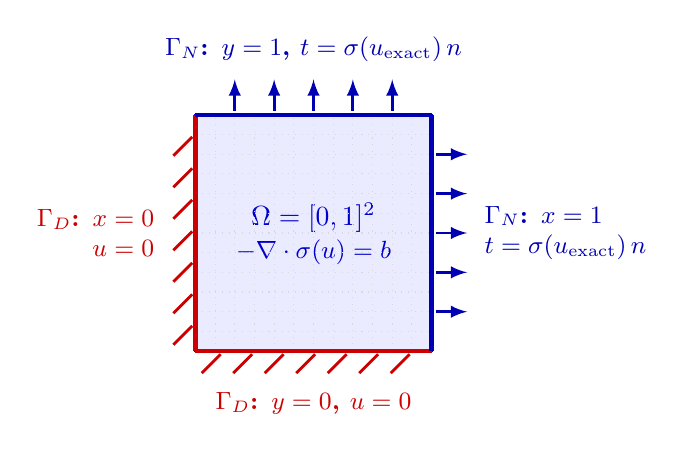
\begin{tikzpicture}[scale=1.0, >=latex]
  % MixedBoundarySinusoidalElasticity2D: 单位正方形, 绘图比例 3 -> 3 x 3
  % Gamma_D: x = 0, y = 0 (位移边界, u = 0); Gamma_N: x = 1, y = 1 (牵引边界, t = sigma n)
  \draw[thick, fill=blue!8, draw=blue!80!black] (0,0) rectangle (3,3);
  \node[font=\bfseries\sffamily, color=blue!80!black, align=center] at (1.5,1.7)
    {$\Omega = [0,1]^2$};
  \node[font=\small, color=blue!80!black] at (1.5,1.25) {$-\nabla\cdot\sigma(u) = b$};

  % Grid overlay
  \draw[step=0.25, gray!30, dotted] (0,0) grid (3,3);

  % Gamma_D: left and bottom, displacement u = 0 (hatched)
  \draw[ultra thick, red!80!black] (0,0) -- (0,3);
  \draw[ultra thick, red!80!black] (0,0) -- (3,0);
  \foreach \y in {0.2, 0.6, 1.0, 1.4, 1.8, 2.2, 2.6} {
    \draw[line width=1.0pt, red!80!black] (-0.28, \y-0.12) -- (-0.04, \y+0.12);
  }
  \foreach \x in {0.2, 0.6, 1.0, 1.4, 1.8, 2.2, 2.6} {
    \draw[line width=1.0pt, red!80!black] (\x-0.12, -0.28) -- (\x+0.12, -0.04);
  }
  \node[left, red!80!black, font=\small\bfseries, align=right] at (-0.4,1.5)
    {$\Gamma_D$: $x = 0$\\$u = 0$};
  \node[below, red!80!black, font=\small\bfseries, align=center] at (1.5,-0.4)
    {$\Gamma_D$: $y = 0$, $u = 0$};

  % Gamma_N: right and top, traction t = sigma n from the exact stress
  \draw[ultra thick, blue!70!black] (3,0) -- (3,3);
  \draw[ultra thick, blue!70!black] (0,3) -- (3,3);
  \foreach \y in {0.5, 1.0, 1.5, 2.0, 2.5} {
    \draw[->, blue!70!black, line width=1.0pt] (3.05,\y) -- (3.45,\y);
  }
  \foreach \x in {0.5, 1.0, 1.5, 2.0, 2.5} {
    \draw[->, blue!70!black, line width=1.0pt] (\x,3.05) -- (\x,3.45);
  }
  \node[right, blue!70!black, font=\small\bfseries, align=left] at (3.55,1.5)
    {$\Gamma_N$: $x = 1$\\$t = \sigma(u_{\mathrm{exact}})\,n$};
  \node[above, blue!70!black, font=\small\bfseries, align=center] at (1.5,3.55)
    {$\Gamma_N$: $y = 1$, $t = \sigma(u_{\mathrm{exact}})\,n$};
\end{tikzpicture}
\end{document}
